\chapter{FlexTouch Working Principles}
\label{flextouch-working-principles}

Any conductive object in contact with the touchscreen draws currents passing from the driving line (transmitting electrode) to the sensing line (receiving electrode) at each junction. The control IC of the touchscreen is designed to measure this leaking current to detect touch events. Prior work introduced an extension tape enlarging the transmitting electrode to boost the touch sensing distance ~\cite{Kato2015, Kato2015a,mobicom-gao18, Ikematsu-Ohmic-Touch}. In Kato's work, the signal transmitted into the conductive tape returns to the device through an environmental coupling path, called \textbf{\textit{virtual ground}}. To further extend the capacitive sensing distance, we introduce the ground of the phone, the \textbf{\textit{local ground}}, into the extended circuit. Therefore, we can short this coupling path with another conductive tape directly passing the signal back to the touchscreen device. Although the local ground can be extended from the charging port, we use the back panel of the touchscreen device since it's easier to assemble as illustrated in Fig ~\ref{fig:plugandplay} C. We can simplify the structure made of the attached conductive tape, the back panel, and the inner local ground circuit as one large capacitor. Here, we define two types of extension strips: 1) \textbf{\textit{signal strip}}, which is attached to the touchscreen sensor node, and 2) \textbf{\textit{grounding strip}} which extends the local ground of the touchscreen.

\begin{figure}[ht]
\centering
    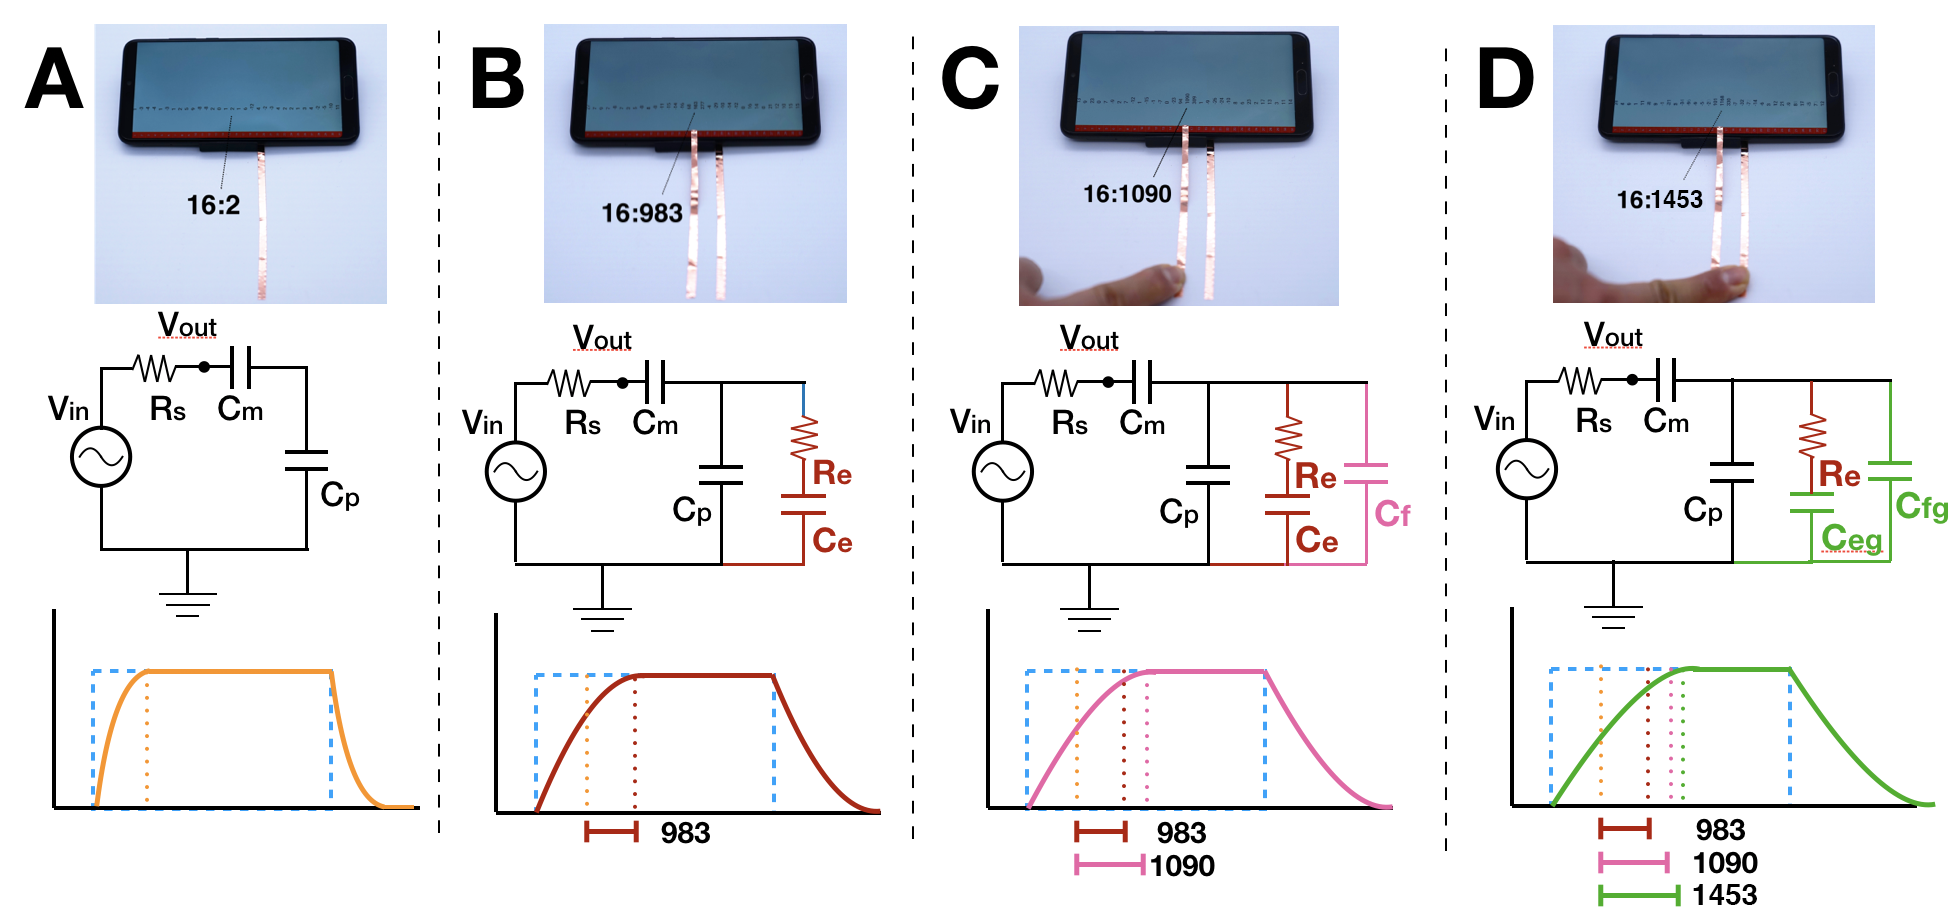
\includegraphics[width=0.75\columnwidth]{figures/principle_mode.png}
    \setlength{\belowcaptionskip}{-8pt}
    \caption{Four capacitive states and corresponding simplified equivalent circuits of \textit{FlexTouch}. A: Idle state - original touchscreen sensing node. B: Attaching state - adding the signal strip on one touchscreen sensing node. C: Touching state - touch on the signal strip. D: Grounding state - touch both the signal strip and the grounding strip.}
    \label{fig:mode}
\end{figure}

We present simplified equivalent circuits under each column in Fig ~\ref{fig:mode} with each capacitive sensor node treated as a RC circuit. $R_{s}$, $C_{m}$, $C_{p}$, $C_{e}$, $C_{f}$, $C_{fg}$,$C_{eg}$, $R_{e}$ represent the inner resistance, mutual capacitance, parasitic capacitance, introduced capacitance between the extended element and local ground, touch introduced capacitance, introduced capacitance of touching both the signal and grounding strips, changed capacitance between the extended element and local ground as well as the extended element introduced resistance. Equation (1) shows the calculation of $v_{out}$ ignoring the effect of $R_{e}$, using $C_{e(g)}$ representing either $C_{e}$ or $C_{eg}$ and $C_{f(g)}$ representing either $C_{f}$ or $C_{fg}$.

\begin{equation}
    V_{out} = v_{in}(1-e^{-\frac{C_{m} + C_{p} + C_{e(g)} + C_{f(g)}}{R_{s}C_{m}(C_{p} + C_{e(g)} + C_{f(g)})}t})
\end{equation}


The touchscreen controller transmits a series of step voltage signals to scan through each electrode and measures the charging time (time for $V_{out}$ to reach a threshold) as raw capacitive values of the touchscreen. The charging time is linearly dependent on the Time Constant of the RC circuit, named $\tau$, that is given as:

\begin{equation}
    \tau = R_{s}\frac{C_{m}(C_{p} + C_{e(g)} + C_{f(g)})}{C_{m} + C_{p} + C_{e(g)} + C_{f(g)}}
\end{equation}

 
We assume that $C_{m}$ and $C_{p}$ are static with value around $10pF$. The value of $C_{e}$ depends on the characteristics of the extended surfaces such as conductivity of the material, length, and width as well as the intersection effect between the extended elements. $C_{f}$ typically varies from several to dozens of $pF$ introduced by human touch. 

Fully understanding the effect of $C_{e}$ is the key to exploring the upper-limit of \textit{FlexTouch}'s performance. In pursuit of testing this limit, we simply model the mutual capacitance between the extended material and the virtual ground with following formula.
% \[C_{e} = \varepsilon \frac{A}{d} = \varepsilon \frac{L \times D}{d} \tag{3}\]

$A$ represents the scale of dimensions of extension strips including length ($L$) and width ($D$), $d$ represents the separation between the signal strip and the local ground, and $\varepsilon$ represents the material's permittivity of extension strips. Therefore, to fully evaluate the sensing distance capability of \textit{FlexTouch}, we need to study the effect of variable factors contained in the fabrication material along with the width and gap distance of the extension strips.